% ============================================================
%  Augmenting Rule-Based Private-Cloud Forensic Investigation
%  with Evidence-Grounded LLM Reasoning
%
%  IEEE conference (double-column) typeset
%  Sources: paper_drafts/00_abstract.md ... 07_conclusion.md
% ============================================================

\documentclass[conference]{IEEEtran}
\IEEEoverridecommandlockouts

\usepackage{cite}
\usepackage{amsmath,amssymb,amsfonts}
\usepackage{graphicx}
\usepackage{textcomp}
\usepackage{xcolor}
\usepackage{booktabs}
\usepackage{array}
\usepackage{verbatim}
\usepackage{url}
\usepackage[hidelinks]{hyperref}
\usepackage{tikz}
\usetikzlibrary{positioning,arrows.meta,shapes.geometric,calc}

% Compact tabular columns for wide comparison tables
\newcolumntype{L}[1]{>{\raggedright\arraybackslash}p{#1}}

\title{Augmenting Rule-Based Private-Cloud Forensic Investigation with Evidence-Grounded LLM Reasoning}

\author{%
  \IEEEauthorblockN{Md.~Nazmul Hasan}
  \IEEEauthorblockA{\textit{Department of Computer Science} \\
  \textit{Institution} \\
  City, Country \\
  email@example.com}
}

\begin{document}
\maketitle

% ------------------------------------------------------------
\begin{abstract}
Private-cloud incident investigation requires reconstructing activity from fragmented authentication, storage, network, web, and administrative logs, without a unified audit plane comparable to public-cloud services. Rule-based correlation provides transparent and auditable triggers but is brittle when evidence is distributed across time and sources. Large language models can synthesise such evidence into investigative narratives, but their forensic use requires that claims be grounded in auditable event references. This paper evaluates an evidence-grounded LLM reasoning pipeline for post-incident forensic triage in a private-cloud setting. The system normalises logs from seven source types into a unified event schema, applies twelve deterministic correlation rules as a transparent baseline, and submits the same timeline to an open-weight LLM that must cite a specific event identifier for every claim. A seven-check validator verifies citation grounding over the LLM output. Across fifteen controlled scenarios, the rule baseline achieved 10/15 binary verdict accuracy (66.7\%) and the LLM achieved 14/15 (93.3\%); the validator recorded no invalid event-ID citations in thirteen of the fifteen scenarios. Failure analysis shows that citation grounding is not equivalent to interpretive correctness: one attack scenario was verdict-correct but attributed to the wrong suspect, and one benign scenario became a false attack verdict that reverses to the correct verdict in a five-run no-rule-context ablation, supporting the hypothesis that rule-alert context amplified the false positive. The results suggest that evidence-grounded LLM reasoning can improve analyst-supervised forensic triage but should not be treated as autonomous detection or attribution.
\end{abstract}

\begin{IEEEkeywords}
digital forensics, post-incident triage, private cloud, large language models, evidence grounding, hallucination mitigation, rule-based correlation, security operations
\end{IEEEkeywords}

% ============================================================
\section{Introduction}
\label{sec:intro}
% ------------------------------------------------------------

Private cloud environments --- organisation-controlled infrastructure operated by banks, government agencies, healthcare providers, and other regulated organisations --- generate forensic evidence across many disjoint surfaces. When an incident occurs and an after-action investigation begins, the analyst must reconstruct what happened from authentication logs, file-access records, administrative actions, network telemetry, database query traces, web-server access logs, and email metadata. Unlike public-cloud platforms, which expose unified audit services such as AWS CloudTrail or Azure Monitor, a private cloud has no single audit plane. The forensic problem is not absence of logs but absence of unified, correlated, investigation-ready evidence. This paper concerns itself with \textbf{post-incident forensic triage} --- timeline reconstruction, evidence-chain analysis, scenario classification, and explanation over already-collected logs --- rather than with real-time intrusion detection.

The dominant industrial approach to triage is rule-based correlation, expressed in SIEM and SOAR platforms as threshold predicates over normalised event streams. Rule-based correlation is transparent, deterministic, and auditable in a way that is essential in regulated settings, but it is brittle in two well-documented directions. It generates large alert volumes on legitimate-but-unusual activity such as travel, conferences, and planned maintenance, and it produces weak verdicts on attacks whose pattern lives in cross-time-window aggregation rather than in any single triggering event. Large language models offer a complementary capability: they can synthesise weak signals across many events, weigh contextual factors such as user role and ticket metadata, and produce narrative explanations of evidence chains. The cost is that an unconstrained LLM can hallucinate evidence, overclaim causality, or attribute an incident to the wrong actor --- failure modes that are unacceptable in forensic contexts where every claim must be defensible against an adversary or in a legal review.

The research question this paper addresses is therefore narrower than the usual ``can an LLM detect attacks?'' framing. We ask: \emph{can an evidence-grounded LLM, operating only over structured normalised events and required to cite specific event identifiers for every claim, improve post-incident forensic triage over a transparent rule-based baseline while preserving traceability?}

The system evaluated in this paper has five components arranged in a single pipeline. First, a normaliser maps logs from seven private-cloud source types --- authentication, file access, administrative, network, database, web server, and email --- onto a unified event schema with explicit event identifiers, timestamps, actors, resources, and metadata. Second, a correlation layer reconstructs a chronologically ordered, session-grouped, cross-source-linked timeline. Third, a deterministic rule engine evaluates twelve threshold-style correlation rules over the timeline and produces a verdict via a transparent severity-mapping function. Fourth, a constrained LLM reasoning layer (Qwen 3.5-27B served through a privately controlled endpoint, replaceable by any OpenAI-compatible local deployment) reads the same timeline and the rule alerts and produces a structured forensic verdict in which every claim must reference one or more event identifiers from the input. Fifth, a seven-check validator inspects the LLM's output for invalid event-ID citations, chronology violations, unsupported actor or entity references, and selected unsupported volume claims. Privacy is treated throughout this paper as a private-cloud deployment constraint --- forensic data does not leave the organisational boundary --- rather than as the headline contribution.

The evaluation comprises fifteen controlled scenarios with predetermined ground truth, organised in two tiers. The primary tier reproduces the four scenarios specified in the original research proposal (a normal baseline, a noisy benign conference-travel case, an obvious external attack, and a slow multi-day insider exfiltration). The extended tier adds eleven robustness scenarios, two of which are documented failure cases. On binary verdict accuracy across all fifteen scenarios, the rule engine is correct on ten (66.7\%), and the evidence-grounded LLM is correct on fourteen (93.3\%). The validator records no invalid event-ID citations in thirteen of fifteen scenarios; in two attack scenarios (S10 and S13) the LLM cited a rule identifier rather than an event identifier in one position, which the validator records as an invalid event-ID reference. These headline numbers conceal an important separation that the paper treats as central. In scenario S14, where a noisy decoy attacker masks a quiet real attacker, the LLM produces the correct binary verdict (\texttt{YES} against an \texttt{ATTACK} ground truth) but identifies the decoy as the suspect --- every event the LLM cites in this scenario is real and chronologically ordered, no event-citation violation is recorded, and the conclusion is wrong about which actor the cited evidence supports. In scenario S15, where legitimate end-of-quarter activity produces ten rule alerts on a benign scenario, the LLM amplifies the rule signal into an incorrect attack verdict; in a five-run no-rule-context ablation (\texttt{data/ablation/S15\_no\_rule\_context.json}, $N=5$, majority verdict \texttt{NO}) the same model on the same timeline returns \texttt{NO}, so the verdict reverses on the presence of the rule-alert artefact alone. S14 is therefore a suspect-attribution failure rather than a verdict failure, while S15 is the lone verdict failure across the corpus. The paper keeps these axes separate throughout.

\subsection{Our Contribution}
\label{sec:contribution}

This paper makes four contributions:

\begin{itemize}
  \item A controlled private-cloud forensic triage benchmark over fifteen incident scenarios using a unified seven-source event schema, with two scenarios designed and retained as adversarial failure cases.
  \item A deterministic rule baseline of twelve transparent correlation rules with a threshold-style verdict mapping, deliberately positioned as an explainable baseline rather than a tuned operational SIEM policy.
  \item An evidence-grounded LLM triage pipeline that restricts the model's reasoning input to normalised events and rule-alert context, requires every claim to cite an event identifier from the input, and validates citation grounding through a seven-check validator covering event-ID existence, chronology, actor and entity consistency, and selected volume claims.
  \item A multi-axis evaluation that separates binary verdict accuracy, suspect and attack-chain correctness, and citation-grounding validity, demonstrating both improvement (66.7\% rule accuracy versus 93.3\% LLM accuracy on verdict, with no invalid event-ID citations in 13 of 15 scenarios and only two stray rule-identifier references in the remaining two) and characterised failure modes (decoy misdirection in S14, rule-context amplification in S15 confirmed by a five-run no-rule-context ablation that reverses the verdict to \texttt{NO}).
\end{itemize}

\subsection{Positioning Against Related Work}
\label{sec:positioning}

Table~\ref{tab:positioning} summarises how this paper's contribution differs from the closest related approaches. Detailed comparison and citations appear in Section~\ref{sec:related}.

\begin{table*}[ht]
\centering
\caption{Comparison of this paper against related approaches.}
\label{tab:positioning}
\small
\begin{tabular}{L{0.16\textwidth}L{0.22\textwidth}L{0.22\textwidth}L{0.30\textwidth}}
\toprule
\textbf{Axis} & \textbf{Rule-based SIEM correlation} & \textbf{Unconstrained LLM analysis} & \textbf{Evidence-grounded LLM triage (this paper)} \\
\midrule
Input & Structured normalised events & Raw or structured logs & Structured normalised events plus rule-alert context \\
Reasoning & Fixed predicates and thresholds & Free-form generation & Constrained scenario reasoning over cited events \\
Evidence grounding & Rule-matched events only & Often weak or absent & Event-ID citation required for every claim \\
Hallucination control & Not applicable & Prompt-only or absent & Seven-check validator over output \\
Private-cloud deployment & Established & Often closed-API-dependent & Open-weight model on a privately controlled endpoint \\
Subtle multi-day pattern & Limited (rules trigger locally) & Potentially yes, unmeasured & Evaluated directly on S4 and S13 \\
Benign noisy activity & Often produces large alert volume & Potentially yes, unmeasured & Evaluated directly on S2, S6, S7, S15 \\
Failure modes & Reported partially & Often hidden & S14 (suspect attribution) and S15 (verdict) explicitly analysed \\
\bottomrule
\end{tabular}
\end{table*}

The remainder of this paper is organised as follows. Section~\ref{sec:background} provides background on private-cloud forensic triage and on the role of rule-based and LLM-assisted reasoning. Section~\ref{sec:related} reviews related work across SIEM correlation, LLM-assisted security operations, LLM-assisted forensics, retrieval-augmented and evidence-grounded generation, and insider-threat detection. Section~\ref{sec:method} describes the system: the normalised event schema, timeline reconstruction, the twelve-rule engine, the LLM reasoning layer, and the validator. Section~\ref{sec:results} reports results across the fifteen scenarios on three orthogonal correctness axes. Section~\ref{sec:discussion} discusses what the LLM contributes beyond rules, the citation-grounding-versus-causal-correctness distinction exposed by S14, the rule-context contamination effect exposed by S15, the implications for forensic triage deployment, and threats to validity. Section~\ref{sec:conclusion} concludes and identifies future directions.

% ============================================================
\section{Background}
\label{sec:background}
% ------------------------------------------------------------

This section defines the terms used throughout the paper and the boundary between forensic triage and real-time detection. It does not repeat the system description in Section~\ref{sec:method} or the related-work synthesis in Section~\ref{sec:related}; it establishes the vocabulary on which both depend.

\subsection{Private-Cloud Forensic Investigation}
\label{sec:bg-pc}

A \emph{private cloud} in this paper denotes self-managed infrastructure operated by a single organisation: virtualised compute, internal storage, on-premises identity providers, internal databases, application servers, and the network fabric that connects them. Banks, government agencies, healthcare providers, and other regulated organisations frequently operate private clouds because their compliance posture or threat model precludes data leaving organisational control. The forensic challenge that follows is not absence of logs --- modern hypervisors, operating systems, and applications produce logs in volume --- but absence of a unified audit plane comparable to public-cloud services such as AWS CloudTrail, Azure Monitor, or Google Cloud Audit Logs. Authentication events live in one system, file-access events in another, network telemetry in a third, and administrative actions and email metadata in still others. After an incident, the investigator's task is to reconstruct what happened from these fragmented surfaces, often days or weeks after the underlying activity occurred. \emph{Forensic investigation} in this paper denotes that reconstruction problem: identifying suspicious evidence chains, classifying the scenario as benign or attack, and producing an account that an analyst, auditor, or legal reviewer can defend.

\subsection{Forensic Triage versus Real-Time Detection}
\label{sec:bg-triage}

Real-time detection and post-incident triage are sometimes conflated, but they differ in input, latency, and operational expectation. Real-time detection operates on streaming events, runs continuously at low latency, and produces alerts that may trigger automated responses such as session termination or network blocking. Triage operates on already-collected logs, runs in batches or on demand after an incident or audit trigger, and produces an investigative output that a human analyst reviews before any action is taken. The system described in this paper is a triage system. It does not generate live alerts, does not block attacks, and does not act autonomously. It assumes that logs have been collected and stored, and its task is to reconstruct, classify, and explain. This boundary is preserved throughout the rest of the paper, and it constrains what the empirical results in Section~\ref{sec:results} can and cannot claim: scenario-level verdict accuracy under controlled conditions is a triage metric, not a detection metric.

\subsection{Rule-Based Correlation}
\label{sec:bg-rules}

Rule-based correlation is the standard industrial approach to converting normalised event streams into security signals. A correlation rule is a deterministic predicate over event fields, optionally combined with thresholds and temporal windows: a single-event predicate such as ``log-deletion action by any user,'' a threshold predicate such as ``more than five file-download events from the same user within thirty minutes,'' or a temporal sequence predicate such as ``privilege-change event followed by a file-download event by the same user within thirty minutes.'' Each firing rule produces an alert that names the rule, the cited events, and a severity. Rules are deterministic, transparent in the sense that their predicate trace can be inspected, and auditable in the sense that an analyst can explain every alert by reference to the rule that fired and the events it matched. The cost is brittleness: rules are sensitive to threshold choice, generate false positives on legitimate edge cases such as travel or planned maintenance, and cannot easily aggregate evidence across time windows long enough that no single rule can hold the whole pattern. The transparent threshold-style rule engine described in Section~\ref{sec:rules} is an instance of this paradigm and is used in this paper as a baseline rather than as a system being defended.

\subsection{LLM-Assisted Forensic Reasoning}
\label{sec:bg-llm}

A large language model offers capabilities that complement rule-based correlation along three axes. The first is temporal synthesis: given a long, structured timeline, an LLM can in principle aggregate weak signals across many events and across time windows that no single rule encodes, producing an account that names the pattern rather than only the individual triggering events. The second is contextual disambiguation: given user role information, ticket metadata, file-type indicators, and travel notes, an LLM can in principle distinguish elevated activity that has a benign explanation from elevated activity that does not --- a distinction that thresholds alone cannot capture. The third is cross-source explanation: given evidence from heterogeneous source types, an LLM can in principle produce a narrative that connects authentication, file-access, and network signals into a single investigative thread.

These capabilities come with risks that are particularly acute in forensic settings. \emph{Hallucination} refers to outputs that are not supported by the input --- invented events, fabricated timestamps, or actors that did not appear in the evidence. \emph{Over-attribution} refers to claims that go beyond what the evidence supports, such as asserting an actor's intent when only their actions are observable. \emph{Prompt sensitivity} refers to the well-documented finding that the same model on the same input can produce qualitatively different outputs depending on the prompt structure, which undermines the reproducibility expectation of forensic science. An LLM applied to forensic evidence without explicit constraint on what it may say, and without a check on whether what it said is supported by the input, is therefore not directly useful for triage. The role of evidence grounding is to convert the LLM's reasoning capabilities into outputs that can be defended.

\subsection{Evidence Grounding and Citation Validation}
\label{sec:bg-grounding}

The remainder of the paper depends on a precise definition of evidence grounding. \emph{In this paper, evidence grounding means that each reported attack-chain step must cite normalised event identifiers that exist in the scenario evidence; it does not mean that the interpretation drawn from those events is necessarily correct.} The model is required to attach an \texttt{event\_id} reference to every step of its attack chain, every item in its supporting and counter-evidence lists, and any narrative claim of fact. \emph{Citation validation} is then a deterministic post-hoc check that every cited identifier resolves to a real event in the input timeline, that the chronology of cited events is consistent with the model's claims, that any actor or entity named in the output appears in the cited events, and that selected volume claims (file counts, transferred bytes) are consistent with the cited events.

Two scopes of correctness must be distinguished from the outset because the rest of the paper turns on the difference. \emph{Citation grounding} --- the property that every cited reference resolves to a real piece of evidence --- is what citation validation enforces. \emph{Interpretive grounding} --- the property that the cited evidence actually supports the claimed conclusion --- is a strictly stronger property, and it is not enforced by citation validation. An adversary who can place plausible-looking events in the evidence stream can satisfy citation grounding while still misdirecting an analyser that relies only on it. An LLM that reads rule alerts as suggestive context can produce a verdict consistent with the alerts but inconsistent with the underlying timeline, and still satisfy every citation check. Citation validation is therefore necessary but not sufficient for forensic correctness, and the empirical results reported in Sections~\ref{sec:results} and~\ref{sec:discussion} are organised around exactly that gap.

% ============================================================
\section{Related Work}
\label{sec:related}
% ------------------------------------------------------------

This work sits at the intersection of five research threads: rule-based security monitoring and SIEM correlation, large language models in security operations, LLM-assisted digital forensics, retrieval-augmented and evidence-grounded generation, and behavioural insider-threat detection. Each thread has produced relevant prior art individually; what remains underexplored is a controlled forensic-triage setting in which deterministic rules and evidence-grounded LLM reasoning are evaluated side by side over the same normalised event schema, with failures separated into verdict, suspect-attribution, and citation-grounding categories. The remainder of this section reviews each thread and concludes with the gap this paper addresses.

\subsection{Rule-Based Security Monitoring and SIEM Correlation}

Rule-based correlation is the dominant industrial approach to security monitoring. SIEM and SOAR platforms encode threshold predicates and temporal correlation rules over normalised event streams, providing deterministic triggers, transparent predicate traces, and auditability --- qualities that are essential in regulated environments. The well-documented cost of this approach is alert volume. Tariq et al.~\cite{ref1} survey alert fatigue in security operations centres and characterise it as a structural rather than incidental problem: rules tuned to minimise false negatives generate an alert volume substantially in excess of what human analysts can investigate, and the correlation layer compounds rather than relieves the problem when rule logic is poorly maintained or the underlying log streams are inconsistent. Ban et al.~\cite{ref2} propose an AI-assisted SIEM framework intended to suppress benign alert clusters before analyst review, using machine learning over alert metadata; the framing is adjacent to ours but does not address evidence-grounded reasoning over the underlying timeline.

Our work treats rule-based correlation as a baseline and as a source of structured evidence for the LLM, rather than as a competitor. The transparent threshold-style rule engine described in Section~\ref{sec:rules} is deliberately weaker than a tuned operational SIEM policy, so the comparison reported in Section~\ref{sec:results} is against an explainable baseline of the kind operators can audit, not against the strongest possible rule configuration. The S15 contamination effect documented in Section~\ref{sec:rule-context} is a direct consequence of including rule output as input context to the LLM, and identifies a calibration gap not addressed in~\cite{ref2}.

\subsection{Large Language Models for Security Operations}

The application of LLMs to security operations has emerged rapidly between 2023 and 2025. Habibzadeh et al.~\cite{ref3} provide a comprehensive survey of LLM use in SOCs across log analysis, triage automation, alert summarisation, and threat-hunting workflows. They observe that most published systems are evaluated on bespoke datasets with bespoke metrics, and that the field lacks shared evaluation infrastructure --- a concern this paper inherits and addresses indirectly through the published, scenario-level evaluation harness described in Section~\ref{sec:eval-setup}.

Singh et al.~\cite{ref4} report a longitudinal empirical study of forty-five SOC analysts over ten months, capturing 3,090 LLM queries in production analytic workflows. They find that LLMs are used predominantly for sensemaking and context-building rather than for high-stakes determinations, and that analysts treat LLM output as a flexible cognitive aid rather than as an autonomous classifier. This finding is central to the deployment posture argued in Section~\ref{sec:implications}: an evidence-grounded LLM is appropriate as a triage assistant whose output is reviewed by a human investigator, not as a final attribution authority. The S14 misdirection result (Section~\ref{sec:failures}) reinforces the same conclusion from the failure-mode side.

\subsection{LLMs for Digital Forensics and Incident Reconstruction}

The thread closest to this paper is LLM-assisted digital forensics. Studiawan, Breitinger and Scanlon~\cite{ref5} propose a standardised methodology and reference dataset for LLM-based timeline analysis, modelled on the NIST Computer Forensic Tool Testing programme. Their headline empirical finding --- that the same model swings dramatically in evaluated performance depending on prompt structure (BLEU 0.15 under cold prompting versus BLEU 0.95 under context-primed prompting on the same timeline) --- implies that arguments about LLM forensic capability are often arguments about prompting rather than about model capability. They also flag five limitations that this paper inherits directly: context-window truncation, closed-model dependence, weak surface metrics, single-host scope, and the absence of a separate hallucination metric. Our system addresses the last of these explicitly through the validator described in Section~\ref{sec:validator}, while the first four define the boundary of our claims (Section~\ref{sec:threats}).

Loumachi and Ghanem~\cite{ref6} propose GenDFIR, a framework that combines rule-based artefact selection with retrieval-augmented LLM reasoning over digital forensic timelines. GenDFIR is the most directly comparable system in the literature: like ours, it pairs deterministic rule logic with an LLM operating over structured evidence; unlike ours, it does not separate verdict accuracy from suspect attribution and grounding integrity in evaluation, and does not explicitly characterise failure modes. Our work differs in three ways: the validator described in Section~\ref{sec:validator} enforces event-ID citation, chronology, and entity-consistency checks before LLM output is accepted; the evaluation harness reports verdict accuracy, suspect correctness, and citation-grounding integrity as separate metrics rather than collapsing them into a single accuracy number; and two failure cases (S14, S15) are kept in the corpus and analysed rather than removed.

Two further contributions complete this thread. The DFIR-Metric benchmark~\cite{ref7} proposes a broad evaluation dataset for LLMs in DFIR with multiple sub-tasks; it is complementary to our narrower controlled private-cloud forensic-triage scope. Yin et al.~\cite{ref8} survey the broader role of LLMs in digital forensics and articulate a structural reproducibility tension: LLMs are inherently probabilistic and can produce variable outputs under identical input, undermining the reproducibility expectation of forensic science. We cite this concern directly in our reproducibility threats to validity (Section~\ref{sec:threats}), and constrain it operationally through low-temperature inference and the citation validator. An earlier survey-style contribution by Wickramasekara et al.~\cite{ref9} explores the potential of LLMs for improving forensic investigation efficiency and provides a useful early framing for the area.

\subsection{Retrieval-Augmented Generation and Evidence-Grounded LLMs}

A separate but technically central thread is retrieval-augmented generation and evidence grounding. Our system is not classical document RAG --- the LLM is given structured normalised events rather than retrieved free-text documents --- but the architectural pattern of supplying external evidence and requiring the model to cite it is identical, and the failure modes documented in this thread map directly onto our results.

Huang et al.~\cite{ref10} survey hallucination phenomena in large language models and propose a taxonomy that distinguishes input-conflicting, context-conflicting, and fact-conflicting hallucinations from intrinsic and extrinsic categories. Our checked-versus-uncovered breakdown in Section~\ref{sec:grounding} is consistent with their taxonomy and makes explicit which categories the validator in Section~\ref{sec:validator} covers (event-ID existence, chronology, entity consistency, selected volume claims) and which it does not (causal overclaim, missing alternative explanation, wrong-suspect-with-grounded-evidence). Sharma~\cite{ref11} surveys retrieval-augmented architectures and notes the now-familiar finding that citation correctness --- every cited source exists --- is necessary but not sufficient for output reliability, because a model can cite real sources and still draw an unsupported conclusion. The S14 result in Section~\ref{sec:failures} is the forensic-domain instance of exactly this distinction: every cited event is real, the validator is silent, and the conclusion is wrong about which actor the cited evidence supports.

\subsection{Insider Threat and Multi-Day Behavioural Detection}

Insider-threat detection has a longer history rooted in behavioural anomaly detection over user activity logs, often evaluated against the synthetic CERT dataset. Tuor et al.~\cite{ref12} propose a deep-learning approach to unsupervised insider-threat detection over structured cybersecurity data streams; this and similar machine-learning baselines establish that multi-day behavioural patterns can be learned from sequence data without explicit rule encoding. More recently, the OrgForge-IT benchmark~\cite{ref13} proposes a verifiable synthetic dataset for evaluating LLM-based insider-threat detection; its framing --- verifiable synthetic ground truth coupled with LLM evaluation --- is closest to ours, although it does not separate verdict from suspect-attribution failures in the way this paper does. Our subtle-attack scenario S4 and the seven-day exfiltration scenario S13 are positioned against this thread: the rule baseline in Section~\ref{sec:subtle} fails on both at the verdict level, while the LLM identifies the multi-day read-then-download pattern that defines them.

\subsection{Gap Addressed by This Paper}

Prior work has examined SIEM alert fatigue, AI-assisted SOC triage, LLM-assisted forensic analysis, and RAG-style evidence grounding. However, these strands do not fully evaluate deterministic rules and evidence-grounded LLM reasoning side by side over the same normalised forensic event schema. This paper addresses that gap by separating binary verdict accuracy, suspect and attack-chain correctness, and citation-grounding validity, showing that an LLM can improve triage accuracy while still failing through grounded but incorrect interpretation.

Table~\ref{tab:related-positioning} summarises how our work positions against each thread.

\begin{table*}[ht]
\centering
\caption{Positioning of this paper against related work threads.}
\label{tab:related-positioning}
\small
\begin{tabular}{L{0.18\textwidth}L{0.22\textwidth}L{0.22\textwidth}L{0.28\textwidth}}
\toprule
\textbf{Work area} & \textbf{Typical approach} & \textbf{Limitation for this paper's question} & \textbf{How this paper differs} \\
\midrule
Rule-based SIEM correlation~\cite{ref1,ref2} & Threshold predicates, temporal correlation rules, alert prioritisation via metadata & Brittle under contextual ambiguity; alert volume hides verdict-level FP/FN behaviour; not designed for cross-time-window aggregation & Used as transparent baseline and as structured evidence input to an LLM, with rule-context contamination measured (S15) \\
LLMs for SOC operations~\cite{ref3,ref4} & Survey + empirical analyst studies; LLMs as flexible cognitive aids & Predominantly real-time / streaming analyst workflows; minimal evidence-grounding enforcement & Post-incident triage focus; explicit citation validator; failure cases preserved and analysed \\
LLMs for digital forensics~\cite{ref5,ref6,ref7,ref8,ref9} & Forensic timeline analysis with prompt-engineered LLMs, with or without rule pre-selection & Grounding rarely enforced operationally; verdict / suspect / grounding failures not separated in evaluation & Validator enforces event-ID citation and consistency; evaluation reports verdict, suspect, and grounding axes separately \\
RAG and evidence grounding~\cite{ref10,ref11} & Retrieval over documents with required source citations; hallucination taxonomy and metrics & Citation correctness $\neq$ causal correctness; document-RAG framing assumes free-text evidence & Structured-event citation rather than document RAG; S14 demonstrates grounded-but-wrong interpretation \\
Insider threat / multi-day behavioural~\cite{ref12,ref13} & Behavioural anomaly detection on CERT or synthetic logs; recently LLM-assisted variants & Verdict-only metrics typical; suspect attribution rarely separated from verdict accuracy & Two scenarios (S4, S13) explicitly target multi-day patterns rule mapping returns BENIGN on; suspect attribution scored separately \\
\bottomrule
\end{tabular}
\end{table*}

The novelty defended by this paper is therefore methodological rather than algorithmic: a controlled comparison between deterministic rule-based triage and evidence-grounded LLM reasoning, over the same normalised forensic event schema, with three orthogonal correctness axes --- verdict, suspect, citation grounding --- and with two characterised failure cases (decoy misdirection and rule-context amplification) that bound where the approach currently breaks.

% ============================================================
\section{Methodology}
\label{sec:method}
% ------------------------------------------------------------

This section describes the forensic triage pipeline used to evaluate rule-based and LLM-assisted reasoning over private-cloud evidence under identical inputs. The pipeline is deliberately simple: it ingests synthetic logs from heterogeneous sources, normalises them into a common schema, reconstructs a correlated timeline, and submits the same structured evidence in parallel to a deterministic rule engine and a constrained open-weight LLM. Both outputs are then evaluated against predetermined ground truth, and the LLM output is additionally validated for evidence-grounding violations.

\subsection{System Overview}
\label{sec:overview}

The pipeline consists of nine stages, executed sequentially per scenario, as illustrated schematically in Fig.~\ref{fig:pipeline}.

\begin{figure}[ht]
\centering
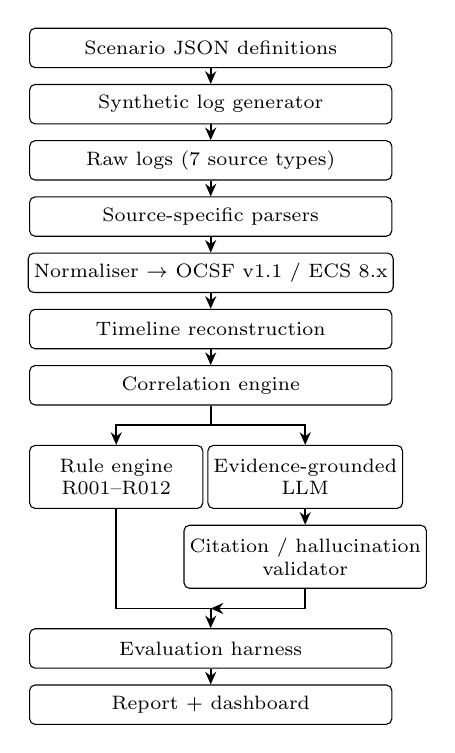
\begin{tikzpicture}[
  node distance=2mm and 4mm,
  every node/.style={font=\scriptsize},
  stage/.style={draw, rectangle, rounded corners=2pt, minimum width=46mm, minimum height=5mm, align=center, inner sep=2pt},
  branch/.style={draw, rectangle, rounded corners=2pt, minimum width=22mm, minimum height=8mm, align=center, inner sep=2pt},
  arr/.style={-{Stealth[length=1.6mm,width=1.4mm]}, semithick}
]
\node[stage] (scen) {Scenario JSON definitions};
\node[stage, below=of scen] (gen) {Synthetic log generator};
\node[stage, below=of gen] (raw) {Raw logs (7 source types)};
\node[stage, below=of raw] (par) {Source-specific parsers};
\node[stage, below=of par] (norm) {Normaliser $\to$ OCSF v1.1 / ECS 8.x};
\node[stage, below=of norm] (tim) {Timeline reconstruction};
\node[stage, below=of tim] (corr) {Correlation engine};

\node[branch, below=5mm of corr.south, xshift=-12mm] (rule) {Rule engine\\R001--R012};
\node[branch, below=5mm of corr.south, xshift=12mm]  (llm)  {Evidence-grounded\\LLM};
\node[branch, below=2mm of llm] (val) {Citation / hallucination\\validator};

\node[stage, below=5mm of val.south, xshift=-12mm] (eval) {Evaluation harness};
\node[stage, below=of eval] (rep)  {Report + dashboard};

\draw[arr] (scen) -- (gen);
\draw[arr] (gen)  -- (raw);
\draw[arr] (raw)  -- (par);
\draw[arr] (par)  -- (norm);
\draw[arr] (norm) -- (tim);
\draw[arr] (tim)  -- (corr);

\coordinate (split) at ($(corr.south)+(0,-2.5mm)$);
\draw[semithick] (corr.south) -- (split);
\draw[arr] (split) -| (rule.north);
\draw[arr] (split) -| (llm.north);

\draw[arr] (llm) -- (val);

\coordinate (merge) at ($(eval.north)+(0,2.5mm)$);
\draw[arr] (rule.south) |- (merge) -- (eval.north);
\draw[arr] (val.south)  |- (merge);
\draw[arr] (eval) -- (rep);
\end{tikzpicture}
\caption{Pipeline overview. Synthetic logs from seven source types are normalised onto a unified event schema, correlated into a chronological timeline, and submitted in parallel to a deterministic rule engine and an evidence-grounded LLM. The validator inspects only the LLM output for citation-grounding violations.}
\label{fig:pipeline}
\end{figure}

Stage boundaries produce structured JSON artefacts that are persisted to disk and reloaded by the next stage. This makes any stage independently testable, reproducible from saved intermediate state, and inspectable for failure analysis. The implementation evaluated in this paper corresponds to commit \texttt{6c7ffbc}, with rule definitions, prompt constraints, validator checks, and schema fields taken directly from the executable pipeline.

\subsection{Log Sources}
\label{sec:logsources}

Seven log source types are ingested. The choice reflects the typical evidence surface available in self-managed private-cloud environments where no unified audit plane exists.

\begin{table}[ht]
\centering
\caption{Log source types and example evidence captured.}
\label{tab:sources}
\small
\begin{tabular}{L{0.22\columnwidth}L{0.70\columnwidth}}
\toprule
\textbf{Source type} & \textbf{Example evidence captured} \\
\midrule
auth        & login, logout, login\_failed (with source IP and authentication method) \\
file\_access & file\_read, file\_download (with resource path and size in bytes) \\
admin       & privilege\_change, log\_delete (with target, justification metadata) \\
network     & dns\_query, firewall\_allow / firewall\_block, vpn\_connect \\
database    & db\_query, db\_login, db\_export, db\_login\_failed \\
web\_server  & http\_request, http\_error (method, URL, status code) \\
email       & mail\_sent (sender, recipients, attachments) \\
\bottomrule
\end{tabular}
\end{table}

Each source type retains its own raw field naming and semantics in \texttt{data/raw\_logs/}, so the parser layer must explicitly map each source's idioms onto the unified schema rather than assuming homogeneous structure.

\subsection{Normalised Event Schema}
\label{sec:schema}

All seven source types are mapped onto a single unified event record. The schema is deliberately minimal so that rule logic and LLM reasoning operate over the same representation:

\begin{verbatim}
{
  "event_id":   "evt_s4_001",
  "timestamp":  "2026-04-01T09:00:00+06:00",
  "source_type":"auth | file_access | admin
                | network | database
                | web_server | email",
  "user":       "user_03",
  "action":     "login | logout | file_read |
                file_download |
                privilege_change |
                log_delete | dns_query | ...",
  "resource":   "/data/finance/reports/",
  "source_ip":  "192.168.1.103",
  "status":     "success | failure",
  "session_id": "sess_user_03_20260401_001",
  "severity":   "info | warning | critical",
  "metadata":   { "ticket": "HR-2026-441",
                  "justification":
                  "Annual review preparation" }
}
\end{verbatim}

All timestamps carry a timezone offset (UTC+6 for the modelled organisation in Dhaka, Bangladesh). Ground-truth fields used to evaluate the system are kept in a separate ground-truth file rather than the events themselves; metadata keys prefixed with an underscore are stripped during normalisation to prevent leakage of evaluation hints into either the rule engine or the LLM input. In addition to the unified schema, each event is mapped to the OCSF v1.1 and ECS 8.x representations to support interoperability with industry SIEM tooling, although the experiments in this paper use only the unified schema.

\subsection{Timeline Reconstruction and Correlation}
\label{sec:timeline}

Normalised events are sorted chronologically and grouped along three orthogonal axes that together produce the input to both downstream analysers.

The first axis is \textbf{session grouping}: events sharing a \texttt{session\_id} are collected into per-session sequences, which surfaces session-level patterns such as mid-session source-IP changes (an indicator of session hijacking) without requiring the analyser to discover sessions itself. The second axis is \textbf{per-user grouping}, used by rules that aggregate events over time windows (for example, counting failed logins within a rolling five-minute window). The third axis is \textbf{cross-source linking}, in which events that share a user and fall within a temporal proximity window are joined across source types --- so that a \texttt{privilege\_change} admin event and a subsequent \texttt{file\_download} file-access event by the same user become a single evidence chain for rules and LLM alike.

The correlator does not attempt heuristic attack-step labelling. It produces a chronologically ordered, lightly grouped event list that preserves all original fields. This is important: the LLM reasons over the same structured data the rule engine sees, not a richer derived representation, so any improvement attributable to the LLM cannot be explained by the LLM receiving privileged input.

\subsection{Rule Engine}
\label{sec:rules}

The rule engine implements twelve detection rules covering the categories conventionally seen in SIEM correlation: anomalous authentication context, threshold-based volume anomalies, privilege misuse, deletion of forensic artefacts, multi-source correlation, and protocol-level indicators. Rules are declared in YAML and evaluated against the normalised event stream and per-user baselines.

\begin{table}[ht]
\centering
\caption{The twelve rules in the rule baseline.}
\label{tab:rules}
\small
\begin{tabular}{L{0.06\columnwidth}L{0.30\columnwidth}L{0.14\columnwidth}L{0.40\columnwidth}}
\toprule
\textbf{ID} & \textbf{Name} & \textbf{Severity} & \textbf{Trigger condition (informal)} \\
\midrule
R001 & unusual\_login\_ip & warning  & login from an IP not in user's normal\_ips \\
R002 & off\_hours\_access & warning  & timestamp outside user's normal\_hours \\
R003 & privilege\_escalation & critical & any privilege\_change action \\
R004 & bulk\_download & critical & $>5$ file\_download events in 30 min \\
R005 & cross\_department\_access & warning & resource directory not in user's normal\_directories \\
R006 & log\_deletion & critical & any log\_delete action \\
R007 & failed\_login\_spike & warning & $\geq 2$ failures in 5 min \\
R008 & privilege\_then\_download & critical & privilege\_change followed by file\_download within 30 min \\
R009 & dns\_tunnel\_detection & critical & $>20$ DNS queries to same domain in 5 min \\
R010 & sql\_injection\_attempt & critical & web event status 500 with SQL keywords in URL \\
R011 & data\_exfiltration\_volume & critical & outbound bytes $>100$ MB in 30 min \\
R012 & lateral\_movement & warning  & same user authenticated against $\geq 3$ server types in 30 min \\
\bottomrule
\end{tabular}
\end{table}

Each scenario yields a list of rule alerts, each tagged with the rule that fired, the severity, and the cited event identifiers. A scenario-level rule verdict is derived from the alert set using a fixed mapping (no critical alerts $\rightarrow$ no\_alert; only warnings $\rightarrow$ suspicious; one or more critical alerts $\rightarrow$ attack). The mapping is intentionally simple so that the rule engine's behaviour is fully transparent and any improvement from the LLM is attributable to reasoning, not to richer rule post-processing. This baseline represents a transparent threshold-style triage engine rather than a tuned SIEM policy optimised per scenario; the comparison reported in this paper is therefore against an explainable rule baseline of the kind operators can audit, not against the strongest possible rule configuration.

\subsection{LLM Reasoning Layer}
\label{sec:llm}

The LLM does not see raw logs. In the headline experimental condition reported in this paper, it receives three structured artefacts: the per-user baselines, the correlated normalised timeline for the scenario, and the list of rule alerts that fired. We refer to this as the \textbf{rule-context condition}. A second \textbf{no-rule-context condition}, in which the rule-alert artefact is omitted, is run as a diagnostic ablation rather than a parallel headline experiment; it is run for S15 over five repetitions, and the canonical artefact is saved at \texttt{data/ablation/S15\_no\_rule\_context.json} with the per-run records under the same directory (discussed in Section~\ref{sec:rule-context}). All headline accuracy figures in this paper refer to the rule-context condition unless explicitly stated otherwise. The LLM is required to produce a forensic verdict in a fixed JSON schema covering: a binary \texttt{verdict} (\texttt{YES}, \texttt{NO}, or \texttt{INSUFFICIENT}), an explicit \texttt{incident\_occurred} boolean, the most suspicious user, an ordered attack chain in which every step cites an \texttt{event\_id}, separate lists of supporting and counter-evidence event identifiers, evidence gaps, and a self-rated confidence with rationale.

The system prompt enforces five strict rules: only events explicitly listed in the timeline may be reasoned over; events may not be assumed, invented, or inferred; insufficient evidence must be reported as such; every claim must reference one or more \texttt{event\_id}s from the input; and every claim carries a confidence label of HIGH, MEDIUM, or LOW. A second block of analysis guidance disambiguates situations the rule engine handles poorly: failed-login bursts without a subsequent successful login do not constitute a breach; legitimate maintenance activity may include privilege changes, log rotation, off-hours work, and bulk file operations and should be cross-checked against role and metadata; ticket justifications can be fabricated and a multi-day read-then-download pattern across departments remains suspicious even when each individual day looks benign; and a mid-session change of source IP within a single \texttt{session\_id} is a strong session-hijacking indicator.

The model used is Qwen 3.5-27B (\texttt{fusion-brain}) served through Modal as a privately controlled remote endpoint. The client is a thin HTTP wrapper over an OpenAI-compatible chat-completions API and is endpoint-agnostic. Substituting an on-premises vLLM, Ollama, or TGI deployment requires only a configuration change to the endpoint URL; the rest of the pipeline is unaffected. This is what makes the architecture compatible with private-cloud deployments where forensic data must not leave the security boundary, but in this paper privacy is treated strictly as a deployment constraint, not as a measured contribution.

\subsection{Evidence-Grounding Validator}
\label{sec:validator}

Every accepted LLM output is passed through a deterministic validator before it is used in evaluation. The validator does not assess whether the LLM's reasoning is correct in a forensic sense; it only enforces that LLM claims are tied to evidence actually present in the input. Seven check categories are implemented (Table~\ref{tab:validator}).

\begin{table}[ht]
\centering
\caption{Validator check categories.}
\label{tab:validator}
\small
\begin{tabular}{L{0.32\columnwidth}L{0.60\columnwidth}}
\toprule
\textbf{Check} & \textbf{What it enforces} \\
\midrule
Event reference existence & Every \texttt{event\_id} cited in attack chain, evidence-for, or evidence-against lists exists in the scenario's normalised timeline. \\
Timeline correctness & Cited events appear in non-decreasing timestamp order. \\
Unsupported claim count & Counts attack-chain steps lacking an \texttt{event\_id}, and tests whether the \texttt{narrative} field contains at least one \texttt{evt\_*} reference; structural, not a general assertion scanner. \\
Actor reference consistency & Any user named in the verdict, suspect field, or narrative appears in the input timeline. \\
Temporal claim validation & ``Within $X$ minutes'' / ``after $Y$'' claims are checked against actual timestamp deltas. \\
Volume claim validation & Claims involving file counts, total volume, or ``large download'' are checked against the size and count of cited events. \\
Entity consistency & Files, IP addresses, and other named entities in the narrative appear in the cited events. \\
\bottomrule
\end{tabular}
\end{table}

The validator's remit is intentionally narrow. It catches \textbf{invalid event-ID citations}, \textbf{chronology violations}, \textbf{unsupported actor or entity references}, and \textbf{selected unsupported volume claims}. It does not address two important hallucination categories: causal overclaiming (asserting a user \emph{intended} exfiltration, where intent is not directly verifiable from logs) and missing alternative explanations (failing to surface plausible benign accounts of the evidence). It also does not assess whether the LLM has identified the \emph{correct} suspect, even when every cited event is real --- a distinction that matters in S14, where the cited evidence is grounded but pertains to a decoy. These categories are discussed qualitatively in Section~\ref{sec:results} rather than scored automatically. The paper's main grounding claim is therefore deliberately bounded: across thirteen of fifteen scenarios the implemented validator records no invalid event-ID citations, with the remaining two scenarios each containing one stray rule-identifier reference --- not ``hallucination-free.''

\subsection{Scenario Design}
\label{sec:scenarios}

Evaluation uses fifteen controlled scenarios with predetermined ground truth, organised in two tiers. The primary tier reproduces the four scenarios specified in the original research proposal and carries the headline narrative of the paper. The extended tier adds eleven robustness and stress scenarios, two of which are documented failure cases that we treat as findings rather than embarrassments.

\textbf{Primary evaluation.}

\begin{table}[ht]
\centering
\caption{Primary evaluation scenarios.}
\label{tab:primary-scenarios}
\small
\begin{tabular}{L{0.20\columnwidth}L{0.16\columnwidth}L{0.52\columnwidth}}
\toprule
\textbf{Scenario} & \textbf{Label} & \textbf{Purpose} \\
\midrule
S1 --- Normal baseline & BENIGN & Both systems should produce no alert; establishes that the pipeline does not cry wolf. \\
S2 --- Noisy benign (conference travel) & BENIGN & False-positive resistance test. Senior developer working from a foreign IP at unusual hours, with elevated download volume, but with travel context and authorised cross-project access. \\
S3 --- Obvious external attack & ATTACK & Sanity check. Compromised credentials, off-hours foreign-IP login, privilege escalation, bulk download, and partial log cleanup. \\
S4 --- Slow multi-day insider & ATTACK & Key scenario. HR specialist incrementally expands access to finance and engineering over three days, shifting from reads to downloads, with a plausible-looking ticket on day one. \\
\bottomrule
\end{tabular}
\end{table}

\textbf{Extended evaluation.} S5 (session hijack with mid-session IP change), S6 (planned maintenance window with legitimate privilege changes and log rotation --- the hardest false positive in the corpus), S7 (failed credential stuffing without breach), S8 (full-infrastructure attack involving SQL injection, database export, and DNS-tunnel exfiltration), and S9--S13 add further coverage of multi-server activity, delayed event arrival, and contradictory evidence.

Two scenarios are deliberately treated as failure cases for the LLM and reported as such. Because they fail along different axes, we keep them separate in all reporting:

\begin{itemize}
  \item \textbf{S14 --- Decoy misdirection (qualitative reasoning failure, not a verdict failure).} A noisy decoy user generates rule-flagging activity while a quiet real attacker performs lateral movement and source-code exfiltration in parallel. The LLM produces the verdict \texttt{YES} against an \texttt{ATTACK} ground truth --- that is, the binary verdict is \emph{correct} --- but identifies the decoy as the suspect and assembles its attack chain from the decoy's events. Every event the LLM cites is real and present in the input, so the validator records no invalid citation. The failure is therefore one of suspect identification and attack-chain interpretation, not of evidence grounding.
  \item \textbf{S15 --- Rule-context amplification (verdict failure, ablation-confirmed).} Legitimate end-of-quarter activity produces a high volume of rule alerts. In the rule-context condition, the LLM amplifies the rule signal into an incorrect \texttt{YES} verdict against a \texttt{BENIGN} ground truth. A five-run no-rule-context ablation on the same model and the same timeline returns \texttt{NO} on all five runs (canonical artefact at \texttt{data/ablation/S15\_no\_rule\_context.json}, summary at \texttt{data/ablation/S15\_ablation\_summary.json}); the verdict therefore reverses on the presence of the rule-alert artefact alone, supporting the rule-context-amplification hypothesis. This is the only verdict-level failure observed across the fifteen scenarios in the headline rule-context condition.
\end{itemize}

For headline accuracy figures, the binary verdict (\texttt{YES} / \texttt{NO} / \texttt{INSUFFICIENT}) is scored against the scenario's \texttt{BENIGN} / \texttt{ATTACK} ground truth label. By that metric the LLM is correct on fourteen of fifteen scenarios (S15 is the lone failure). Suspect identification and attack-chain correctness are scored separately and are where S14 fails. Conflating these two metrics would obscure the result; the Results and Discussion sections preserve the distinction.

The two-tier structure is intentional. The primary four scenarios anchor the paper's main claim against the originally proposed scope; the extended eleven provide robustness coverage and the two documented failure cases delimit where evidence-grounded LLM reasoning still breaks.

% ============================================================
\section{Results}
\label{sec:results}
% ------------------------------------------------------------

\subsection{Evaluation Setup}
\label{sec:eval-setup}

The evaluation comprises fifteen controlled scenarios over the unified event schema described in Section~\ref{sec:method}. Five scenarios carry the ground-truth label \texttt{BENIGN} (S1, S2, S6, S7, S15) and ten carry the label \texttt{ATTACK} (S3, S4, S5, S8, S9, S10, S11, S12, S13, S14). Both systems run against the same normalised timeline per scenario; the LLM additionally receives the rule-engine alert list as part of the rule-context condition described in Section~\ref{sec:llm}.

Three families of metrics are reported. \textbf{Verdict accuracy} is the binary classification of the scenario as \texttt{BENIGN} or \texttt{ATTACK}. \textbf{Suspect and attack-chain correctness} measure whether the LLM identified the right primary actor and assembled an evidence chain consistent with the ground-truth attack steps. \textbf{Evidence-grounding integrity} counts validator violations across the seven check categories defined in Section~\ref{sec:validator}. We keep the three families separate throughout, because the most important findings of the paper --- S14 and S15 --- fail along different axes and would be obscured if collapsed into a single accuracy number.

All figures in this section are computed by the evaluation harness from saved per-scenario LLM responses, rule-engine outputs, and validator results.

\subsection{Scenario-Level Verdict Accuracy}
\label{sec:verdict-accuracy}

The headline result is summarised in Table~\ref{tab:verdict}.

\begin{table}[ht]
\centering
\caption{Verdict accuracy across 15 scenarios.}
\label{tab:verdict}
\small
\begin{tabular}{L{0.46\columnwidth}cc>{\raggedleft\arraybackslash}p{0.14\columnwidth}}
\toprule
\textbf{System} & \textbf{Correct} & \textbf{Total} & \textbf{Accuracy} \\
\midrule
Rule engine (transparent threshold baseline) & 10 & 15 & 66.7\% \\
LLM (rule-context condition) & 14 & 15 & \textbf{93.3\%} \\
Invalid event-ID citations (validator) & 2 & 243 & 0.8\% \\
\bottomrule
\end{tabular}
\end{table}

The rule engine produces the correct binary verdict on ten of fifteen scenarios. The five scenarios where rules fail at the verdict level are S5 (concurrent lateral movement), S6 (legitimate after-hours maintenance, where rules fire on multiple critical patterns and yield an \texttt{attack} verdict against a \texttt{BENIGN} ground truth), S10 (delayed and out-of-order events), S12 (conflicting signals), and S13 (ultra-slow exfiltration over seven days). The LLM produces the correct verdict on fourteen of fifteen scenarios; the lone verdict failure is S15 (end-of-quarter legitimate bulk activity), discussed in Section~\ref{sec:failures}. In four of the five scenarios where rules fail (S5, S10, S12, S13), the LLM is correct --- and on S6, the hardest false positive in the corpus, the LLM is also correct.

These numbers describe binary verdict performance only. They do not address suspect identification, attack-chain quality, or hallucination behaviour --- which are reported separately below. The improvement margin over rules ($\approx 27$ percentage points) holds against an explicitly transparent rule baseline; a tuned operational SIEM policy would likely close part of this gap, and the paper does not claim otherwise.

\subsection{False-Positive Reduction}
\label{sec:fp-reduction}

False positives are counted at two granularities: at the \textbf{verdict level} (system declares an \texttt{ATTACK} on a \texttt{BENIGN} scenario) and at the \textbf{alert level} (individual rule firings on benign-scenario events). Table~\ref{tab:fp} reports both for the five benign scenarios.

\begin{table*}[ht]
\centering
\caption{False positives on benign scenarios.}
\label{tab:fp}
\small
\begin{tabular}{L{0.06\textwidth}L{0.22\textwidth}c c c c c}
\toprule
\textbf{Scenario} & \textbf{Description} & \textbf{Rule alerts} & \textbf{Rule verdict (mapped)} & \textbf{FP --- Rules} & \textbf{LLM verdict} & \textbf{FP --- LLM} \\
\midrule
S1  & Normal baseline                & 0          & BENIGN & No  & NO  & No \\
S2  & Noisy travel (conference)      & 13         & BENIGN & No  & NO  & No \\
S6  & After-hours maintenance        & \textbf{33} & ATTACK & \textbf{Yes} & NO  & No \\
S7  & Failed credential stuffing     & 20         & BENIGN & No  & NO  & No \\
S15 & End-of-quarter legitimate bulk & 10         & BENIGN & No  & YES & \textbf{Yes} \\
\bottomrule
\end{tabular}
\end{table*}

Across the five benign scenarios the rule engine generates 76 alert-level false positives in aggregate --- 33 of them on S6 alone. The verdict-level mapping absorbs many of these (the \texttt{suspicious} rule verdict is mapped to \texttt{BENIGN}), which is why the rule engine's verdict accuracy on benign scenarios remains four out of five despite the alert-level noise. The LLM, by contrast, generates only one verdict-level false positive (S15) and matches the ground truth on the other four benign scenarios --- including S6, where the rule engine's verdict is wrong.

The most operationally relevant comparison is on S2, S6 and S7. On S2 (a senior developer travelling to a conference, with an unfamiliar IP, late-night work, elevated download volume, and authorised cross-project access) and S7 (sustained failed login attempts that never produce a successful login), rules generate enough alerts to attract analyst attention while the LLM correctly returns \texttt{NO}. On S6, rules return an outright \texttt{ATTACK} verdict; the LLM returns \texttt{NO}. These three scenarios are where the LLM's contextual reasoning over the same evidence visibly reduces analyst burden.

\subsection{Subtle Attack Recognition}
\label{sec:subtle}

The paper's central empirical claim is that an evidence-grounded LLM, given structured private-cloud evidence, recognises attacks whose pattern is only visible in aggregate across time. The four scenarios that exercise this capability most directly are S4, S5, S10 and S13.

S4 (slow multi-day insider) is the originally-proposed key scenario. An HR specialist gradually expands access into finance and engineering across three days, shifts from reads to downloads, and produces a plausible-looking ticket on day one. The rule engine returns \texttt{attack} (driven primarily by the privilege change and cross-department access rules), so on S4 the rule engine is verdict-correct. However, the rule alert set captures only the privilege event and the cross-department reads; the downstream multi-day read-then-download pattern that constitutes the actual exfiltration is not represented in any single rule. The LLM, given the full timeline, returns \texttt{YES} and reconstructs an attack chain that names the multi-day scope-creep pattern explicitly. F1 against the ground-truth attack steps is 0.10 for the rule engine and 0.91 for the LLM on this scenario.

S5 (concurrent activity with lateral movement) involves a session-hijack pattern where the source IP changes mid-session. The rule engine fires only three alerts and yields a \texttt{suspicious} verdict, mapped to \texttt{BENIGN} --- a verdict-level miss against \texttt{ATTACK} ground truth. The LLM correctly identifies the mid-session IP change and returns \texttt{YES}, with rule F1 of 0.86 and LLM F1 of 0.92.

S10 (delayed and out-of-order events) exercises whether either system tolerates timestamp disorder. The rule engine fires three alerts, yielding \texttt{suspicious} (mapped to \texttt{BENIGN}, verdict-level wrong against \texttt{ATTACK}). The LLM identifies the attack despite the disordered timeline.

S13 (ultra-slow exfiltration over seven days) is the longest-horizon attack in the corpus. Rule alerts are sparse (six in total) and their verdict maps to \texttt{BENIGN}; the LLM returns \texttt{YES}. This is the clearest example in the corpus of an attack pattern that lives entirely in cross-day aggregation rather than in any single triggering event.

These four scenarios are where the difference between the two systems is largest. On S5, S10 and S13, the rule engine is verdict-wrong; the LLM is verdict-right.

\subsection{Evidence-Grounding Validation}
\label{sec:grounding}

Across all fifteen scenarios, the validator described in Section~\ref{sec:validator} recorded \textbf{no invalid event-ID citations in 13 of 15 scenarios}. Of 243 total event-identifier references made by the LLM across the corpus, 241 resolve to real events in the input timeline. The two exceptions occur in S10 and S13, where the LLM's \texttt{evidence\_for} list includes \texttt{R005} --- a rule identifier --- in one position alongside otherwise valid \texttt{evt\_*} references; the validator flags these as invalid event-ID citations. Chronology violations occurred in two of fifteen scenarios (S4 and S5), where the LLM ordered one attack-chain step out of timestamp sequence; the cited events were real, but the order in which they appear in the chain does not strictly follow their timestamps. Actor-reference checks recorded zero violations: every user named in a verdict, suspect field, or narrative appears in the input. Entity-consistency checks recorded one violation, in S12, where the LLM's narrative names an IP address (\texttt{192.168.1.100}) that does not appear in any cited event; the cited events themselves are real, but the IP referred to in the prose is not present in their fields. Volume- and temporal-claim checks were not exercised in any of the fifteen accepted outputs because the LLM did not phrase claims in forms that triggered those checks; we therefore neither claim nor measure their behaviour. The validator additionally records 15 unsupported claims across the corpus (one per scenario), reflecting attack-chain steps or narrative sentences that lack an explicit \texttt{evt\_*} reference; these are structural artefacts of the response template rather than fabricated evidence.

Table~\ref{tab:grounding} reports grounding results by hallucination type, distinguishing what the validator covers from what it does not.

\begin{table}[ht]
\centering
\caption{Grounding results by hallucination type.}
\label{tab:grounding}
\small
\begin{tabular}{L{0.40\columnwidth}L{0.22\columnwidth}L{0.28\columnwidth}}
\toprule
\textbf{Hallucination type} & \textbf{Coverage} & \textbf{Observed} \\
\midrule
Nonexistent event-ID citation & Full & 2 (S10, S13) \\
Chronology violation & Full & 2 (S4, S5) \\
Unsupported actor reference & Full & 0 \\
Unsupported entity reference (IP / file) & Full & 1 (S12) \\
Unsupported volume claim & Selected fields & Not exercised \\
Unsupported temporal claim & Selected fields & Not exercised \\
Unsupported chain or narrative claim (missing \texttt{evt\_*}) & Structural & 15 (one per scenario) \\
Causal overclaim (e.g.\ asserted intent) & Not covered & Discussed (Section~\ref{sec:failures}) \\
Missing alternative explanation & Not covered & Discussed (Section~\ref{sec:failures}) \\
Wrong-suspect identification with grounded evidence & Not covered & 1 (S14, Section~\ref{sec:failures}) \\
\bottomrule
\end{tabular}
\end{table}

The bounded scope is the point. The validator catches the hallucination types where forensic claims must not appear out of thin air. It does not assess whether a grounded claim points to the \emph{right} event, the \emph{right} actor, or the \emph{right} causal interpretation --- and the S14 failure case exists precisely in that gap.

\subsection{Failure Cases}
\label{sec:failures}

\subsubsection*{S14 --- Decoy misdirection (qualitative reasoning failure, validator-silent)}

S14 simulates two simultaneous attacks. A loud decoy compromise on user\_04 generates twenty-one rule alerts: brute-force authentication, privilege escalation, and bulk downloads. Concurrently, the real attack is a quiet lateral movement against user\_02, exfiltrating proprietary source code over DNS tunnelling from an internal IP. The ground-truth attacker is user\_02. The LLM returns the verdict \texttt{YES} against an \texttt{ATTACK} ground truth --- so the binary verdict is correct --- but identifies user\_04 as the suspect and assembles its attack chain entirely from user\_04's events. Every event the LLM cites is real and present in the timeline, so no validator check fires.

This is the most informative failure in the corpus. It separates two forms of correctness that look similar from a distance but diverge under adversarial evidence: \textbf{citation grounding} (does every cited event exist?) and \textbf{interpretive grounding} (does the cited evidence support the claim?). The implemented validator covers the first and not the second. Evidence grounding in the citation sense is necessary for forensic reasoning but not sufficient. An adversary who can place a decoy in the evidence stream can satisfy citation grounding while still misdirecting the analyser.

The lesson is that evidence-grounded LLM reasoning needs an additional layer that the present system does not implement: multi-suspect hypothesis tracking, with the LLM required to enumerate alternative actors and the evidence for and against each, before settling on a primary suspect. This is taken up in Section~\ref{sec:conclusion}.

\subsubsection*{S15 --- Rule-context amplification (verdict failure)}

S15 simulates legitimate end-of-quarter financial activity. A finance user accesses many sensitive files in a short window because the quarterly close is in progress. The rule engine generates ten alerts, mostly on the \texttt{bulk\_download} and \texttt{cross\_department\_access} rules, and produces a \texttt{suspicious} verdict, which the verdict mapping correctly absorbs to \texttt{BENIGN}. The LLM, however, returns \texttt{YES} against a \texttt{BENIGN} ground truth --- the lone verdict-level LLM failure in the corpus.

A diagnostic ablation removes the rule-alert artefact from the LLM's input and re-runs the same scenario on the same model. Under the no-rule-context condition, the LLM returns \texttt{NO} on all five runs (canonical artefact at \texttt{data/ablation/S15\_no\_rule\_context.json}, summary at \texttt{data/ablation/S15\_ablation\_summary.json}); under the rule-context condition the same model returns \texttt{YES} on all five runs (\texttt{data/ablation/S15\_rule\_context.json}). The verdict therefore reverses unanimously on the presence of the rule-alert artefact alone. The natural reading is that, in the rule-context condition, the LLM treats the rule alerts as quasi-ground-truth signals rather than as candidate evidence to be weighed; ten alerts, even when individually weak, push the model's posterior toward \texttt{ATTACK} enough to flip the verdict.

This characterises a contamination effect rather than a property of the underlying model. It also implies an architectural recommendation that the rest of the literature on hybrid SIEM/LLM systems should attend to: rule output presented to an LLM is not neutral context. It is suggestive context, and on weakly-supported alerts it can override the model's own reading of the timeline. Calibrated rule-context handling --- for example, including rule alerts only with explicit confidence weights, or asking the LLM to score the rule alerts before asking it to render a verdict --- is a clear next step.

\subsubsection*{Causal overclaim and missing alternative explanations}

The validator does not check causal overclaiming. Manual inspection of the fifteen attack-scenario narratives finds occasional sentences asserting user \emph{intent} (e.g.\ ``the user planned to exfiltrate'') that the timeline cannot directly support. These remain a known gap. Similarly, on benign-mapped scenarios the LLM does not reliably enumerate alternative benign explanations even when its verdict is correct; on S15 in the rule-context condition, the absence of an explicit ``this could be quarterly close activity'' hypothesis is part of why the wrong verdict was reached.

\subsection{Summary of Findings}
\label{sec:summary}

\begin{table*}[ht]
\centering
\caption{Findings tied to evidence.}
\label{tab:findings}
\small
\begin{tabular}{L{0.42\textwidth}L{0.32\textwidth}L{0.18\textwidth}}
\toprule
\textbf{Finding} & \textbf{Supporting scenarios} & \textbf{Evidence in this section} \\
\midrule
LLM achieves higher verdict accuracy than transparent rule baseline & 14/15 vs 10/15 across all scenarios & Section~\ref{sec:verdict-accuracy} \\
LLM correctly handles benign-but-noisy activity that produces large rule alert volume & S2, S6, S7 & Section~\ref{sec:fp-reduction} \\
LLM recognises subtle multi-day or cross-time-window attacks where rule mapping returns BENIGN & S5, S10, S13 (and richer narrative on S4) & Section~\ref{sec:subtle} \\
LLM produces no invalid event-ID citations in 13 of 15 scenarios; the remaining two (S10, S13) each contain one stray rule-identifier reference & 13 of 15 & Section~\ref{sec:grounding} \\
Citation grounding is necessary but not sufficient: the LLM can be misdirected by adversarial decoys whose events are real & S14 & Section~\ref{sec:failures} \\
Rule output is not neutral context to the LLM; weak alerts may amplify into incorrect attack verdicts & S15 (no-rule-context ablation, 5/5 runs return \texttt{NO}, reverses verdict unanimously) & Section~\ref{sec:failures} \\
Causal overclaim and missing-alternative-explanation are uncovered hallucination categories & Qualitative across attack scenarios & Section~\ref{sec:failures} \\
\bottomrule
\end{tabular}
\end{table*}

The defended claim, restated against the evidence above:

\begin{quote}
In controlled private-cloud forensic scenarios with known ground truth, an evidence-grounded open-weight LLM improved scenario-level verdict accuracy from 10/15 (66.7\%) to 14/15 (93.3\%) over a transparent threshold-based rule baseline, while producing no invalid event-ID citations in 13 of 15 scenarios under the implemented validator (two scenarios contain one stray rule-identifier reference each, out of 243 total event-identifier references). The improvement is concentrated on subtle multi-day attacks and on benign-but-noisy scenarios. Two characterised failure modes --- adversarial decoy misdirection (S14, suspect-level rather than verdict-level) and rule-context amplification (S15, the lone verdict failure, in which a five-run no-rule-context ablation reverses the verdict to \texttt{NO} on all five runs) --- bound where the approach currently breaks.
\end{quote}

% ============================================================
\section{Discussion}
\label{sec:discussion}
% ------------------------------------------------------------

The empirical results in Section~\ref{sec:results} establish that an evidence-grounded LLM, given the same structured timeline as a transparent rule baseline, raises scenario-level verdict accuracy from 10/15 (66.7\%) to 14/15 (93.3\%) while producing no invalid event-ID citations in 13 of 15 scenarios (two scenarios contain one stray rule-identifier reference each). This section argues that the right reading of those numbers is not ``the LLM detects attacks,'' but a more bounded claim: that the LLM contributes \textbf{contextual interpretation} over evidence the rules already see, and that the contribution comes with characterised failure modes that constrain how the system should be deployed.

\subsection{What the LLM Adds Beyond Rules}
\label{sec:llm-adds}

Both systems consume the same correlated normalised timeline. The rule engine fires deterministic predicates over per-event fields and sliding time windows; the LLM is asked to read the same timeline and produce a verdict, a suspect, an attack chain, and supporting and counter-evidence with \texttt{event\_id} citations. The difference between the two is therefore not a difference of \emph{evidence access} --- it is a difference of \emph{evidence synthesis}.

Three forms of synthesis show up clearly in the results. The first is \textbf{aggregation across time windows that no single rule covers}. S4 (slow multi-day insider) and S13 (ultra-slow exfiltration over seven days) both exhibit attack patterns that exist only in the cross-day pattern of reads-followed-by-downloads, scope creeping outward from the user's own department. No individual rule fires often enough on these scenarios to produce a critical verdict; on S13, only six rule alerts fire across seven days, and the rule verdict mapping returns \texttt{BENIGN}. The LLM, given the entire timeline, identifies the read-then-download progression and returns \texttt{YES}. The contribution here is not detection in the usual sense; it is \emph{temporal aggregation that the rule engine architecturally cannot perform.}

The second is \textbf{contextual downgrading}. On S2 (a senior developer at a conference, twenty cross-project file accesses with a foreign IP and elevated download volume) and on S6 (a sanctioned maintenance window with privilege changes, log rotation, and bulk file operations on configuration paths), the rule engine fires a substantial number of alerts --- thirteen on S2 and thirty-three on S6. The LLM correctly returns \texttt{NO} in both cases because it can read the user role, the metadata fields (ticket numbers, justification text), and the file types, and recognise that the alert pattern is consistent with explainable activity. The contribution here is the inverse of the first: \emph{interpretation that prevents alerts from translating into incidents.}

The third is \textbf{cross-source pattern reading}. S5 (concurrent activity with a mid-session source-IP change) is a session-hijack signal where the rules fire only three weak alerts. The LLM's prompt explicitly tells it to flag mid-session IP changes within the same \texttt{session\_id} as a hijacking indicator; given that guidance and the timeline, it returns \texttt{YES}. This is the smallest of the three contributions in interpretive depth --- the LLM is essentially executing a soft rule the rule engine does not encode --- but it is the most operationally plausible to lift back into the rule engine in future work.

In each case the LLM is doing something a richer rule set could in principle approximate. The point of the experiment is not that an LLM is uniquely capable of these inferences. It is that an evidence-grounded LLM provides them \emph{without requiring an analyst to enumerate every cross-time-window pattern in advance}, and without producing claims that cannot be tied back to specific events.

\subsection{Where Rules Still Matter}
\label{sec:rules-matter}

The same evidence makes it clear that rules are not displaced. They are upstream input.

Rules are deterministic, fast, and auditable in a way the LLM is not. A rule firing on a specific event has a fixed predicate trace and a fixed severity; an LLM verdict has neither. Rules can run continuously against streaming logs at low cost; the LLM is heavyweight and runs against batched, correlated input post-incident. Rules produce alert identifiers that the LLM can cite, which is a structural reason to keep them in the loop: the LLM's attack chain becomes more reviewable when it can point at both rule alerts and underlying events.

The rule baseline reported in this paper is also explicitly a transparent threshold-style triage configuration, not a tuned operational SIEM policy. It is not the strongest possible rule deployment. A real SIEM in production would carry per-rule severity tuning, suppression lists for known maintenance windows, and aggregation policies that would close part of the 27-percentage-point gap reported in Section~\ref{sec:verdict-accuracy}. The paper does not claim that the LLM beats a state-of-the-art SIEM. It claims that, against an explainable baseline that operators can audit, the LLM contributes interpretive synthesis that the rule layer is not architected to produce.

The right architectural reading is therefore not LLM-instead-of-rules. It is LLM-after-rules, with rules providing deterministic triggers, alert candidates, and a bounded input the LLM can cite --- and with the explicit understanding that rule input is suggestive context, not ground truth (see Section~\ref{sec:rule-context}).

\subsection{Grounding Is Necessary but Not Sufficient}
\label{sec:grounding-not-sufficient}

The validator described in Section~\ref{sec:validator} records no invalid event-ID citations in 13 of 15 scenarios; in two scenarios (S10 and S13) the LLM cites a rule identifier rather than an event identifier in one position, which the validator flags. Chronology violations occur in 2 of 15 scenarios (S4 and S5) where one attack-chain step is ordered out of timestamp sequence. Every actor named in any scenario appears in that scenario's input timeline; one entity-consistency violation occurs in S12, where the narrative names an IP address not present in any cited event. Within those bounds, the LLM's output is grounded.

S14 shows what that guarantee does and does not buy. In S14 the ground-truth attacker is user\_02, who exfiltrates source code over DNS tunnelling from an internal IP while user\_04, the decoy, generates twenty-one rule alerts with a loud brute-force-and-download pattern. The LLM returns the correct binary verdict (\texttt{YES} against \texttt{ATTACK}) but identifies user\_04 as the suspect and assembles its entire attack chain from user\_04's events. For S14 specifically, every cited event is real, the chain is chronologically ordered, and no event-ID-citation or chronology violation is recorded. The cited evidence is grounded; the conclusion is wrong about which actor it supports.

This is the most important interpretive result in the paper. \textbf{Citation grounding} --- does every cited event exist? --- is one form of correctness. \textbf{Interpretive grounding} --- does the cited evidence support the chosen conclusion? --- is a different form. The validator covers the first and not the second. An adversary who can place plausible-looking events in the evidence stream can satisfy citation grounding while still misdirecting the analyser. Evidence grounding in the citation sense is necessary for forensic reasoning, but it is not sufficient.

The defended sentence the paper carries forward is therefore deliberately bounded:

\begin{quote}
The system improves forensic triage accuracy under controlled conditions, but evidence-grounded citation validation only prevents unsupported references; it does not guarantee correct causal interpretation or correct suspect attribution.
\end{quote}

S14 is what makes that sentence load-bearing rather than rhetorical. It also implies a concrete extension: the next layer of validation must check whether the cited evidence is \emph{sufficient and exclusive} support for the claimed suspect, not merely whether it exists. Multi-suspect hypothesis tracking --- requiring the LLM to enumerate alternative actors and the evidence for and against each --- is taken up in the Conclusion as a future-work direction.

\subsection{Rule-Context Contamination}
\label{sec:rule-context}

S15 exposes a second, distinct failure mode. End-of-quarter financial activity produces ten rule alerts on a \texttt{BENIGN} scenario. In the rule-context condition (the headline experimental setup), the LLM returns \texttt{YES} against the \texttt{BENIGN} ground truth --- the lone verdict-level LLM failure across the corpus. A no-rule-context ablation runs the same scenario on the same model with the rule-alert artefact removed from the prompt input. Across five runs the no-rule-context condition returns \texttt{NO} on all five (\texttt{data/ablation/S15\_no\_rule\_context.json}, summary at \texttt{data/ablation/S15\_ablation\_summary.json}); under the rule-context condition the same model returns \texttt{YES} on all five (\texttt{data/ablation/S15\_rule\_context.json}). The verdict therefore reverses unanimously on the presence of the rule-alert artefact alone, and the rule-context-amplification hypothesis is supported by the data.

The natural reading is that the LLM treats the rule alerts as a probabilistic signal toward \texttt{ATTACK} rather than as candidate evidence to be weighed and downgraded. Ten alerts, even when each is individually a weak indicator on its own (\texttt{bulk\_download} and \texttt{cross\_department\_access} rules firing on quarter-close volume), are sufficient to push the LLM's posterior past the verdict threshold. The model still cites real events; the validator still records no event-ID-citation violation in S15. The failure is in \emph{how rule context is interpreted}, not in \emph{what is cited}.

This is consistent with a contamination effect of the kind familiar from the broader retrieval-augmented literature: when supplied context carries an implicit verdict signal, the model can inherit that signal even when the underlying evidence does not justify it. For hybrid SIEM/LLM systems, the practical implication --- confirmed by the no-rule-context ablation --- is that \textbf{rule output is not neutral input.} Three architectural responses follow:

\begin{itemize}
  \item \textbf{Calibrated rule-context handling.} Rule alerts should be presented with explicit confidence weights --- high-precision rules differently from broad-recall rules --- so the LLM is not encouraged to treat all alerts as equivalent evidence.
  \item \textbf{Two-stage prompting.} Ask the LLM to first score the rule alerts (which look strong, which look weak, which are explained by the timeline) before asking it to render a verdict. Decouple the alert reading from the verdict reading.
  \item \textbf{Counterfactual ablation as a deployed check.} On any scenario where the rule-context verdict is \texttt{YES}, run a no-rule-context comparison and flag verdict reversals for human review. S15 is the canonical case in which this catches the failure automatically: the rule-context verdict is \texttt{YES}, the no-rule-context verdict is \texttt{NO}, and the disagreement is the operational signal that the analyst should review the alert before acting on it.
\end{itemize}

None of these are research novelties; they are calibration techniques the field has developed for retrieval-augmented systems. The contribution from S15 is the demonstration, supported by saved per-run artefacts, that they apply directly to rule-augmented forensic LLMs.

\subsection{Implications for Forensic Triage}
\label{sec:implications}

The two failure cases together delimit the role the LLM should play. It is not a final attribution authority. It is a constrained reasoning layer that produces a candidate verdict, a candidate attack chain, and a candidate suspect, all tied to specific event citations --- and a human analyst is required to accept, reject, or refine that output. S14 shows this is necessary because citation grounding does not catch wrong-suspect-with-real-evidence. S15 shows it is necessary because rule-alert context influences the verdict in a direction the underlying evidence does not justify (the no-rule-context ablation reverses the verdict on all five runs).

Operationally, the deployment posture this implies is post-incident triage assistance rather than autonomous detection. The system is appropriate for after-action reports, audit response, and tier-1 investigative summarisation --- settings where the LLM's output is reviewed before it informs a decision. It is not appropriate for real-time blocking, automated response actions, or autonomous attribution. The defended-sentence framing makes this explicit: triage accuracy under controlled conditions does not transfer into causal-interpretation guarantees.

A second implication is that the privacy-preserving deployment story (open-weight model running on the organisation's own infrastructure) is \emph{enabled} by this triage-assistant framing rather than the other way around. If the system were claimed as autonomous detection, the privacy property would be a liability --- the organisation would be running a high-stakes classifier whose failure modes it cannot easily inspect. As an analyst-supervised reasoning assistant, the privacy property is straightforward operational hygiene: forensic data does not leave the security boundary, and the analyst remains the decision-maker.

\subsection{Threats to Validity}
\label{sec:threats}

The results in Section~\ref{sec:results} must be qualified along four dimensions.

\textbf{Internal validity.} The fifteen scenarios are author-designed with predetermined ground truth. We wrote both the scenarios and the prompt that the LLM operates under, and we calibrated the latter against early scenario runs. A reviewer's reasonable concern is that the scenarios are partly designed to expose patterns the LLM is good at and the rules are not. The mitigations are partial: the rule baseline is published, the prompts are published, and the failure cases (S14 and S15) are kept in the corpus rather than removed when their results were inconvenient. The transparent rule baseline is also weaker than a tuned SIEM, which makes the comparison fair against an explainable baseline but not against the strongest rule-only configuration available in production.

\textbf{External validity.} The scenarios are synthetic. Real enterprise logs are noisier, sparser in ground-truth labelling, and exhibit a wider variation in user behaviour than the four modelled personas. The unified event schema and the single modelled organisation (Dhaka, UTC+6, four user roles) abstract away cross-organisation heterogeneity. Real-world validation on a public benchmark (LANL authentication, DARPA OpTC) or on anonymised organisational logs is required before any claim about production-grade detection performance can be made.

\textbf{Construct validity.} The headline metric is binary verdict accuracy. This is a coarse construct for what forensic investigators actually need from a triage assistant. F1 against the ground-truth attack-step labels is reported, but it is sensitive to label-naming agreement: on S8 the LLM returns the correct verdict (\texttt{YES}) but the F1 against named attack steps is 0.10 because the LLM uses different terminology than the ground-truth labels for the same events. Verdict accuracy and attack-step F1 thus measure different and partly orthogonal forms of correctness, and neither captures \emph{narrative usefulness} --- whether the LLM's account is genuinely helpful to a human investigator. A human analyst study is the missing piece for this construct, and is identified in future work.

\textbf{Validator scope.} The grounding claim is bounded by what the validator checks. Causal overclaim --- assertions of intent that the timeline cannot directly support --- is uncovered, and manual inspection of the attack-scenario narratives finds occasional intent-attribution sentences that the timeline does not justify. Missing-alternative-explanation is uncovered: on benign scenarios the LLM does not reliably surface alternative benign hypotheses even when its verdict is correct, and on S15 the absence of an explicit ``this could be quarterly close'' hypothesis is part of why the verdict was wrong. Wrong-suspect-with-grounded-evidence is uncovered, and S14 shows it can be exploited adversarially. Each of these is a known gap, and each motivates a specific extension in future work.

\textbf{Reproducibility.} The results depend on a specific model version (Qwen 3.5-27B served via Modal as \texttt{fusion-brain}) and on the published prompt. Temperature is set to 0.1, which is low but not zero, so identical inputs do not guarantee identical outputs across runs; the headline numbers are from a single representative run rather than averaged across many. The endpoint-agnostic architecture means the same prompts and same scenarios can in principle be run against vLLM, Ollama, or TGI deployments of the same weights, but local reproducibility has not been validated end-to-end in this study. Multi-model comparison and run-variance characterisation are both identified as future work.

These four threats together carry a single message that the abstract and conclusion repeat: the contribution of this paper is a controlled-scenario comparison that isolates a specific reasoning behaviour, with characterised failure modes --- not a production-grade detection claim. The defended sentence in Section~\ref{sec:grounding-not-sufficient} is the boundary the paper does not cross.

% ============================================================
\section{Conclusion}
\label{sec:conclusion}
% ------------------------------------------------------------

Private-cloud forensic triage requires evidence synthesis across fragmented log surfaces, and the absence of a unified audit plane in self-managed infrastructure makes this synthesis the central bottleneck for post-incident investigation. This paper compared a deterministic rule baseline and an evidence-grounded large language model reasoning layer under the same normalised event schema, with the LLM constrained to cite specific event identifiers for every claim and validated through a seven-check grounding validator.

Across fifteen controlled scenarios, the rule baseline produced the correct binary verdict on ten and the LLM on fourteen, and the validator recorded no invalid event-ID citations in 13 of 15 scenarios; the remaining two scenarios each contained a single stray rule-identifier reference. The improvement is concentrated on subtle multi-day attacks and on benign-but-noisy activity that produces large alert volume without a corresponding incident.

The same evaluation exposed two limits that bound the contribution. In one scenario the LLM produced the correct binary verdict but identified a decoy actor as the suspect, with every cited event in that scenario still real and chronologically ordered --- a grounded but interpretively wrong conclusion. In another benign scenario the presence of rule-alert context coincided with an incorrect attack verdict; a five-run no-rule-context ablation on the same model and the same timeline reverses the verdict to \texttt{NO} on all five runs, so the verdict reverses on the rule-alert artefact alone, supporting the rule-context-amplification hypothesis. Citation validity does not imply causal correctness, and rule output is not neutral context to a downstream LLM.

The practical implication is not that an LLM should replace forensic analysts or deterministic controls, but that evidence-grounded LLM reasoning can be useful when its outputs are validated, its failure modes are reported, and its role is limited to analyst-supervised triage. Strengthening this role is the natural next step: a larger and more heterogeneous scenario corpus, a human-analyst usefulness study, multi-hypothesis suspect tracking that requires the model to enumerate and weigh alternative actors, and a stronger validator that addresses causal overclaim and missing alternative explanations alongside the citation-grounding categories already covered.

% ============================================================
\begin{thebibliography}{00}

\bibitem{ref1}
Tariq et al.,
``Alert Fatigue in Security Operations Centres: Research Challenges and Opportunities,''
\textit{ACM Computing Surveys}, 2025.
DOI: 10.1145/3723158.

\bibitem{ref2}
Ban et al.,
``Breaking Alert Fatigue: AI-Assisted SIEM Framework for Effective Incident Response,''
\textit{Applied Sciences (MDPI)}, vol.~13, no.~11, 6610, 2023.

\bibitem{ref3}
A.~Habibzadeh, F.~Feyzi, R.~Ebrahimi Atani,
``Large Language Models for Security Operations Centers: A Comprehensive Survey,''
arXiv:2509.10858, 2025.

\bibitem{ref4}
R.~Singh, S.~Tariq, F.~Jalalvand, M.~Baruwal Chhetri, S.~Nepal, C.~Paris, M.~Lochner,
``LLMs in the SOC: An Empirical Study of Human--AI Collaboration in Security Operations Centres,''
arXiv:2508.18947, 2025.

\bibitem{ref5}
H.~Studiawan, F.~Breitinger, M.~Scanlon,
``Towards a Standardized Methodology and Dataset for Evaluating LLM-Based Digital Forensic Timeline Analysis,''
\textit{Forensic Science International: Digital Investigation}, vol.~54, 2025.
arXiv:2505.03100.

\bibitem{ref6}
F.~K.~Loumachi, M.~C.~Ghanem,
``GenDFIR: Advancing Cyber Incident Timeline Analysis Through Retrieval Augmented Generation and Large Language Models,''
arXiv:2409.02572, 2024.

\bibitem{ref7}
B.~Cherif, T.~Bisztray, R.~A.~Dubniczky, A.~Aldahmani, S.~Alshehhi, N.~Tihanyi,
``DFIR-Metric: A Benchmark Dataset for Evaluating Large Language Models in Digital Forensics and Incident Response,''
arXiv:2505.19973, 2025.

\bibitem{ref8}
Z.~Yin, Z.~Wang, W.~Xu, J.~Zhuang, P.~Mozumder, A.~Smith, W.~Zhang,
``Digital Forensics in the Age of Large Language Models,''
arXiv:2504.02963, 2025.

\bibitem{ref9}
A.~Wickramasekara, F.~Breitinger, M.~Scanlon,
``Exploring the Potential of Large Language Models for Improving Digital Forensic Investigation Efficiency,''
\textit{Forensic Science International: Digital Investigation}, vol.~52, 301859, 2025.
DOI: 10.1016/j.fsidi.2024.301859.
arXiv:2402.19366.

\bibitem{ref10}
Huang et al.,
``A Survey on Hallucination in Large Language Models: Principles, Taxonomy, Challenges, and Open Questions,''
\textit{ACM Transactions on Information Systems}, 2025.
DOI: 10.1145/3703155.

\bibitem{ref11}
C.~Sharma,
``Retrieval-Augmented Generation: A Comprehensive Survey of Architectures, Enhancements, and Robustness Frontiers,''
arXiv:2506.00054, 2025.

\bibitem{ref12}
A.~Tuor, S.~Kaplan, B.~Hutchinson, N.~Nichols, S.~Robinson,
``Deep Learning for Unsupervised Insider Threat Detection in Structured Cybersecurity Data Streams,''
in \textit{Proc.\ AAAI Workshop on AI for Cyber Security}, 2017.
arXiv:1710.00811.

\bibitem{ref13}
J.~Flynt,
``OrgForge-IT: A Verifiable Synthetic Benchmark for LLM-Based Insider Threat Detection,''
arXiv:2603.22499, 2026.

\end{thebibliography}

\end{document}
